% Copyright 2004 by Till Tantau <tantau@users.sourceforge.net>.
%
% In principle, this file can be redistributed and/or modified under
% the terms of the GNU Public License, version 2.
%
% However, this file is supposed to be a template to be modified
% for your own needs. For this reason, if you use this file as a
% template and not specifically distribute it as part of a another
% package/program, I grant the extra permission to freely copy and
% modify this file as you see fit and even to delete this copyright
% notice. 

\documentclass{beamer}

% There are many different themes available for Beamer. A comprehensive
% list with examples is given here:
% http://deic.uab.es/~iblanes/beamer_gallery/index_by_theme.html
% You can uncomment the themes below if you would like to use a different
% one:
%\usetheme{AnnArbor}
%\usetheme{Antibes}
%\usetheme{Bergen}
%\usetheme{Berkeley}
%\usetheme{Berlin}
%\usetheme{Boadilla}
%\usetheme{boxes}
%\usetheme{CambridgeUS}
%\usetheme{Copenhagen}
%\usetheme{Darmstadt}
%\usetheme{default}
%\usetheme{Frankfurt}
%\usetheme{Goettingen}
%\usetheme{Hannover}
%\usetheme{Ilmenau}
%\usetheme{JuanLesPins}
%\usetheme{Luebeck}
\usetheme{Madrid}
%\usetheme{Malmoe}
%\usetheme{Marburg}
%\usetheme{Montpellier}
%\usetheme{PaloAlto}
%\usetheme{Pittsburgh}
%\usetheme{Rochester}
%\usetheme{Singapore}
%\usetheme{Szeged}
%\usetheme{Warsaw}


% Customize Warsaw color 
\setbeamercolor*{palette primary}{use=structure,fg=white,bg=red!50!black}
\setbeamercolor*{palette secondary}{use=structure,fg=white,bg=red!60!black}
\setbeamercolor*{palette tertiary}{use=structure,fg=white,bg=red!70!black}

% Customize Warsaw block title and background colors
\setbeamercolor{block title}{bg=red!50!black,fg=white}


% List your packages here

\usepackage[colorinlistoftodos]{todonotes}


\title[]{A Universal Platform for Building Energy Management}

% % A subtitle is optional and this may be deleted
% \subtitle{Product Proposal}

\author[B.~Lauer]{Brian~Lauer\\\and
Advisor: Dr. Suruz Miah}
% - Give the names in the same order as the appear in the paper.
% - Use the \inst{?} command only if the authors have different
%   affiliation.

\institute[Bradley University] % (optional, but mostly needed)
{
  Department of Electrical and Computer Engineering\\
  Bradley University\\
  1501 W. Bradley Avenue\\
  Peoria, IL, 61625, USA
}
% - Use the \inst command only if there are several affiliations.
% - Keep it simple, no one is interested in your street address.

\date[October~25,~2019]{Friday, October~25,~2019}
% - Either use conference name or its abbreviation.
% - Not really informative to the audience, more for people (including
%   yourself) who are reading the slides online

\logo{\hfill\href{http://www.bradley.edu}{
\includegraphics[width=0.75cm]{../figs/logoBU1-Print}}}  % place logo in every page 


\subject{Mobile Robot Localization}
% This is only inserted into the PDF information catalog. Can be left
% out. 

% If you have a file called "university-logo-filename.xxx", where xxx
% is a graphic format that can be processed by latex or pdflatex,
% resp., then you can add a logo as follows:

% \pgfdeclareimage[height=0.5cm]{university-logo}{university-logo-filename}
% \logo{\pgfuseimage{university-logo}}

% Delete this, if you do not want the table of contents to pop up at
% the beginning of each subsection:



% Let's get started
\begin{document}

\begin{frame}
  \titlepage
\end{frame}

\begin{frame}{Outline}
  \tableofcontents
  % You might wish to add the option [pausesections]
\end{frame}

\section{Overview of Idea}

\begin{frame}{Overview of Idea}
\begin{itemize}
\item Control power states of computers remotely on the LAN
\item Reduce power consumption of desktop PCs and/or servers
\item Monitor power consumption using WeMo switch
\end{itemize}
\end{frame}

% Section and subsections will appear in the presentation overview
\section{Wake-on-LAN}
\begin{frame}{Wake-on-LAN}
\begin{itemize}
\item Ability to wake up computer from sleep state or turn on from off state
\item Initiated with a \textit{magic packet} which is a string of $6$ bytes, all $255$ ($0xFFFFFFFFFFFF$), followed by sixteen repetitions of target computers 6-byte MAC address
\end{itemize}
\begin{block}{Cons}
\begin{itemize}
\item Computers can only be turned on
\item Computer will need to be turned off by disconnecting AC power with WeMo Switch
\item Wake on AC can be configured in most BIOS to allow the computer to boot immediately upon reconnection to AC power
\item Requires specific motherboard and NIC
\item Wired network connection needed
\end{itemize}
\end{block}
\end{frame}

\section{IPMI}
\begin{frame}{IPMI}
\begin{itemize}
\item Intelligent Platform Management Interface (IPMI) provides management capabilities independent of the CPU and OS
\item Interacts with Baseboard Management Controller (BMC) to interact with different components of the motherboard and computer
\item Can remotely turn on, turn off, and power cycle servers through LAN connection
\item Monitor system temperature, voltage, and fans 	
\begin{block}{Cons}
\begin{itemize}
\item Only server motherboards are manufactured with BMCs
\item Dedicated network port needed
\item May be very complicated to implement in BEMOSS
\item Will need to purchase dedicated server with BMC
\end{itemize}
\end{block}
\end{itemize}
\end{frame}

\begin{frame}{IPMI}
\begin{figure}
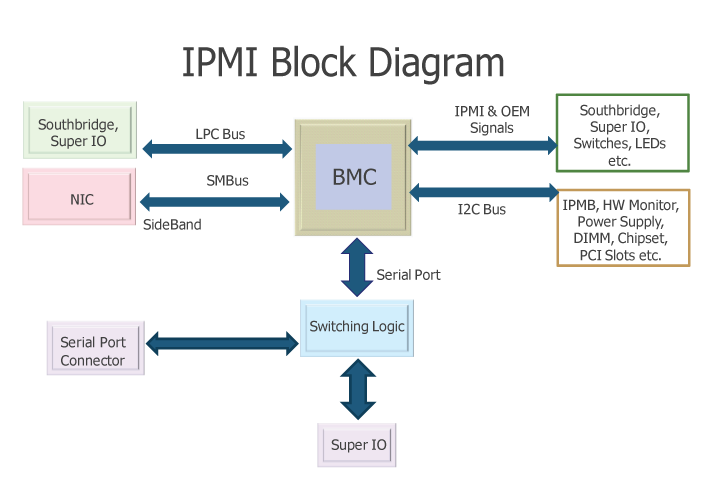
\includegraphics[scale=0.35]{../figs/ipmiBlockDiagram}
\caption{Image taken from \cite{IPMI}}
\end{figure}
\end{frame}

\section*{Summary}
\begin{frame}{Summary}
\begin{itemize}
\item May find different device instead do to the complexity and lack of feasibility of this idea
\item Still need to do a lot of research on this topic
\item Scheduling could be implemented to turn computers/servers on/off at certain points in the day
\end{itemize}
\end{frame}

% All of the following is optional and typically not needed. 
\appendix
\section<presentation>*{\appendixname}
\subsection<presentation>*{For Further Reading}

\begin{frame}[allowframebreaks]
  \frametitle<presentation>{For Further Reading}
    
  \begin{thebibliography}{10}
    
  \setbeamertemplate{bibliography item}[online]
  % Start with overview books.

  \bibitem{openHAB}
  openHAB
  \newblock openHAB site
  \newblock \texttt{https://www.openhab.org}
  
  \bibitem{Wake-on-LAN}
  Wake-on-LAN
  \newblock Wake-on-LAN wiki page
  \newblock \texttt{https://en.wikipedia.org/wiki/Wake-on-LAN}
  
  \bibitem{IPMI}
  IPMI
  \newblock IPMI wiki page
  \newblock \texttt{https://en.wikipedia.org/wiki/
  Intelligent\_Platform\_Management\_Interface}
  \end{thebibliography}
\end{frame}

\begin{frame}
\center
Any Questions?
\end{frame}
\end{document}



%%% Local Variables:
%%% mode: latex
%%% TeX-master: t
%%% End:
